\subsection{GraphDrawer}
To solve the problem of letting students visually answer questions, GraphDrawer was created. GraphDrawer is the name of a VueJS component which is used to display graphics to the user. It is implemented as an software engine (https://en.wikipedia.org/wiki/Software\_engine), which means that it is responsible for rendering the world and handling user interaction. 
\\[11pt]
The world consists of two types of entities, nodes (vertices) and edges. Entities are stored in arrays on the GraphDrawer object. Nodes are drawn as either a circle or a square. A node needs to specify its position in the world, which is stored on the node object as the properties \code{x} and \code{y}. It also needs to store information about how large it is, which is stored in the \code{r} property. \code{r} represents either the circle radius, or the length of each side of the square. A node needs a value, stored in the \code{v} property. This can be text, a number, or a combination of text and numbers. GraphDrawer will only render nodes if they have the \code{x}, \code{y}, \code{r} and \code{v} properties. There are also several optional properties a node can have. \code{selected} is a boolean used by a controller to indicate whether a node has been selected (\code{true}) or not (\code{false}). \code{culled} is a boolean used by the camera to indicate whether a node has been culled (\code{true}) or not (\code{false}). \code{fillColor} decides what color will be used to render the inner part of the node. If it's undefined, white will be used. \code{strokeColor} decides  what color will be used to render the outline of a node. If it's undefined, black will be used. Edges are used to link nodes together. An edge needs to have two properties, \code{n1} and \code{n2}, which are references to the nodes being linked by the edge. Edges are drawn as either a line or an arrow, between the two nodes. If the edge has the property \code{directed} with the value \code{true}, an arrow will be drawn pointing from \code{n1} at \code{n2}. If \code{directed} is \code{false} or \code{undefined}, a line is drawn. The \code{strokeColor} property decides which color will be used to draw the line/arrow. If it's undefined, black is used. An edge can also have the \code{v} property. \code{v} represents the cost of going from \code{n1} to \code{n2} (and from \code{n2} to \code{n1} if \code{directed} is \code{undefined} or \code{false}). \code{v} should be a number, and its value will be drawn next to the line/arrow.
\\[11pt]
To render the world, three objects are needed, the world, a camera and a HTML5 canvas. The world has information about the entities. The camera is used to decide which entities need to be drawn to the canvas. These objects are needed because the world might be larger than what is possible to display on a single webpage. The canvas decides how much of the webpage is used to render the world. The camera can then be moved around to display different parts of the world. When the GraphDrawer starts, an interval is started which lets the GraphDrawer update 60 times every second. Each time the GraphDrawer has the opportunity to update, is called a frame. Because the application is designed to be used by both phones and computers, computationally expensive and time consuming operations should be avoided if possible. For this reason the GraphDrawer will often discard frames. Discarding frames means that no operation is performed, even though the opportunity to do something was there. The update function is called once per frame. If the \code{dirty} property is \code{false}, the frame is discarded. The GraphDrawer will only set the \code{dirty} property to \code{true} once, at startup, so the initial state is rendered. Afterwards a controller has to tell the GraphDrawer to not discard the next frame by setting \code{dirty} to \code{true}. The \code{dirty} property makes it possible to have a responsive user interface, and save CPU time at the same time. When a frame isn't discarded, the world will be redrawn. This is done in several steps:
\begin{enumerate}
    \item The canvas is cleared. This is done to prevent entities to appear at two positions at the same time.
    \item Nodes and edges are drawn to a drawing buffer (\code{drawBuffer}). This is done by the GraphDrawer.
    \item The user interface is drawn to a separate buffer (\code{staticBuffer}). This is done by the GraphDrawer if the \code{operatingMode} is set to \code{Presentation}, or by a controller if the \code{operatingMode} is set to \code{Interactive}. \code{operatingMode} is used by the GraphDrawer and by controllers to decide what kind of user interaction is allowed.
    \item \code{drawBuffer} and \code{staticBuffer} is drawn to the canvas.
\end{enumerate}
The drawing buffer is used to prevent screen tearing (https://en.wikipedia.org/wiki/Screen\_tearing). By using a seperate buffer for drawing, the user will be shown a complete image of the world at every frame, instead of one which is in the process of being drawn. Another buffer is used by the user interface because it makes it easier to draw the interface on top of the world, by simply placing the draw statement after the world draw statement. The \code{staticBuffer} uses canvas coordinates to draw, which needs less operations to consistently place the interface inside the cameras view.
\\[11pt]
To let the user interact with the world two event listeners are attached to the canvas. \code{mousedown} is used to respond to mouse clicks, and \code{touchstart} is used by touch screens. These listeners use the same callback function. The callback function will pass the event to the right handler, depending on handler priority. A handler is a function which takes the event as an argument, and returns whether it consumed the event. If the event was consumed, it should not be given to any other handler. The priority of the user interface handler should generally be higher than the world handler, but the order is not forced. The GraphDrawer will first check if the user interacted with one of the buttons. If not, then a controller will be given the chance to handle the event. Finally, the event is given to the gesture handlers. Gesture handlers are responsible for detecting patterns in user interaction and check if they match a given gesture. The GraphDrawer implements two gestures, pan and zoom. Pan is used to move the camera around the world. A pan gesture happens when the user clicks a mouse button, and moves the pointer without releasing the button. It can also happen if the user drags their finger across the canvas. The movement must be larger than a given threshold before the camera starts moving. A zoom gesture is defined as the user dragging two fingers in opposite directions. If the fingers move towards eachother, the zoom decreases. If the fingers move away from eachother, the zoom increases. The average point between the fingers will remain at the same position relative to the canvas edge. The position of events are stored in different properties of the event object, depending on what type of event it is. To make it simpler to write code that works with all types of events, a helper function \code{setEventOffset} was created to convert event positions to a common format. This function should be used right after recieving a event object, to be sure the position of the event is available in the expected properties.

setEventOffset
\\[11pt]
The controller interface....
\\[11pt]
GraphDrawer configuration...
\\[11pt]
Steps...


\subsubsection{Camera}
The camera object is responsible for letting the user view only a section of the world at a time, and for converting between canvas and world coordinates. The camera object has a position given by the \code{centerX} and \code{centerY} properties. Depending on the canvas size and the \code{zoomLevel} a section of the world will be rendered. To determine if a node or edge should be drawn, the \code{cull(object, isNode)} method is used. It returns \code{false} if the object is inside the camera view, or \code{true} if the object is outside. An culled object should not be drawn. An node is culled if it is outside the camera view. An edge is culled if both nodes are outside the camera view.
!! Insert image showing the relationship between world, camera and canvas coordinates. !!
!! Insert image showing culling. !!

\subsubsection{Graph0}
Graph0 is the controller which is responsible for making it possible to work with graphs and trees. It can be used for both datastructures, because a tree is a graph with some restrictions. Graph0 can also be used to create a Dijkstra task by drawing a graph and marking the start and end nodes. 
!! Insert Graph0 UI Image !!
The Graph0 constructor takes two arguments. The first should be a reference to the GraphDrawer object. The second is an optional configuration object. The following properties can be set from values found in the object.
\begin{enumerate}
    \item \code{exportType}, determines if the drawn graph should be exported as a tree or as a graph. Possible values are \code{"Graph"} and \code{"Tree"}. If no value is given, \code{exportType} is set to \code{"Graph"}.
    \item \code{subType}, determines what kind of algorithm to use. Possible values are \code{"Dijkstra"}. If no value is given, \code{subType} is set to \code{undefined} and no algorithm will be used.
    \item \code{startNodeColor}, determines which fill color the start node is marked with. If no value is given, \code{startNodeColor} is set to a light green color.
    \item \code{endNodeColor}, determines which fill color the end node is marked with. If no value is given, \code{endNodeColor} is set to a light red color.
\end{enumerate}
The Graph0 controller defines five different states, Add, Remove, Move, Join and Edit. Each of them have their own event handler defined by a method in the class. There is also a Mark state which is only available to the user if the \code{subType} is defined.
\begin{enumerate}
    \item Add. The Add state lets the user add a new node to the graph. The new node is placed at the position of interaction event. The value of the node is set to a letter if \code{subType} is set to \code{"Dijkstra"}, or 0 if \code{subType} is undefined. The Add state always consumes the event. 
    \item Remove. The Remove state lets the user remove a node or an edge from the graph. If the interaction event happened inside of a node or close to an edge, it is removed and the event is consumed. If nothing was removed, the event is not consumed. If a node is removed, then any edge connecting the node to another node, is also removed.
    \item Move. The Move state lets the user move a node. This is done using a drag and drop motion. When the interaction starts, a reference to the node under the interaction event is stored. When new events are recieved the position of the node is updated to match the position of the event. The event is consumed only if the first event happened inside a node.
    \item Join. The Join state lets the user create an edge between two nodes. This is done using a drag and drop motion. When the interaction starts, a reference to the node under the interaction event is stored. When the interaction ends, the event handler checks if the is a different node under the event. If another node is found, an edge between this node and the first node is created. The event is consumed only if the first event happened inside a node.
    \item Edit. The Edit state lets the user edit the value of a node or of an edge. The event handler starts by checking if there is a node under the interaction event. If a node is found, the user can edit the value. If no node is found, the handler checks if the event is close to an edge. If it is, the value of the edge can be edited. The event is consumed if the user was given the option to edit a value.
    \item Mark. The Mark state lets the user mark nodes as either a start or end node. If a node is found under the interaction event. It's marked value is updated bases on its current value. A unmarked node is marked as the start node. A start node is marked as the end node. A end node is set to unmarked. The event is consumed if a node changed its marked value.
\end{enumerate}

\subsubsection{Sort}
The Sort controller lets user perform the Quicksort and Mergesort algorithms on arrays.
\begin{figure}[H]
    \centering
    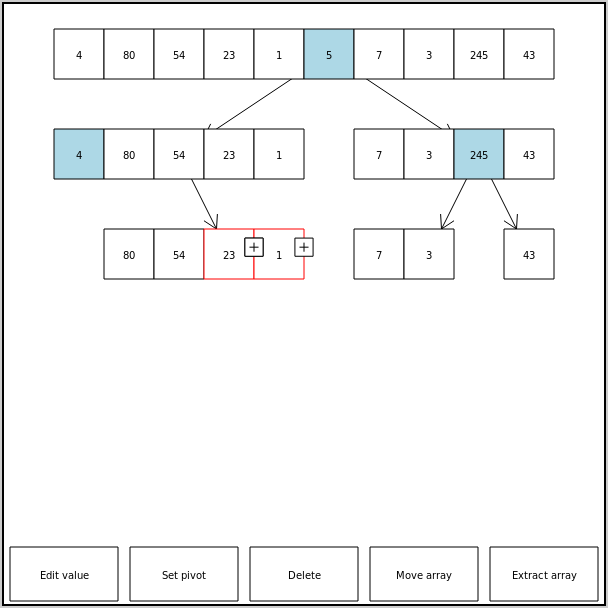
\includegraphics[width=0.75\linewidth]{/graphdrawer/sortui}
    \caption{Sort - user interface}
    \label{fig:graphdrawerSortUserInterface}
\end{figure}
The following properties can be determined by the optional configuration object:
\begin{enumerate}
    \item \code{sortType}, determines which algoritm to use. Can either be \code{"Mergesort"} or \code{"Quicksort"}. The default value is \code{"Quicksort"}.
    \item \code{bsf}, button-size-factor, determines how large the "+" buttons between nodes are. The default value is 3.
    \item \code{pivotColor}, determines which fill color nodes which are marked as pivot will have.
    \item \code{selectedColor}, determines which stroke color nodes which are selected will have.
    \item \code{extractType}, determines node position relative to other nodes when extracting nodes from an array. Possible values are \code{"vSorter"} which means the nodes are positioned based on their value, from low to high, and \code{"xSorter"} which poisitions them based on their x-position in the world.
    \item \code{joinType}, determines node position relative to other nodes when joining the nodes from different arrays to a new array. Possible values are \code{"vSorter"} and \code{"xSorter"}.
    \item \code{steps}, which contains information about the starting array which the student needs to sort. It can also contain information about all of the actions one of the algorithms perform to sort the array.
\end{enumerate}
The \code{mouseDownHandler} function has four parts. It will first check if the world is empty. If it is, the first click will create the first node and array. If it is not empty, then it will check if any of the buttons were clicked. The buttons can only be clicked if they are visible, and they are made visible when the user selects one or more nodes. Only one node can be marked as \code{selected} (marked by + buttons \ref{fig:graphdrawerSortUserInterface}), but several can be in the selection list (marked by a red border \ref{fig:graphdrawerSortUserInterface}). When the user selects a node, the "Edit value", "Set pivot" and "Delete" buttons are shown. If the selection list contains node from only one array, the "Move array" and "Extract array" buttons are also shown. If the \code{sortType} is \code{"Mergesort"} and the selection list contains nodes from at least one array, then the "Join" button is also shown. If no button is clicked, and the user is trying to move an array, the array will be moved to the position of the interaction event. Finally, if nothing else happened, the selected node and the selection list is updated based on which nodes the user interacts with. When the user clicks and holds down their mouse button, the controller will start tracking which nodes are under the cursor. When the button is released, any node which was under the cursor will be in the selection list, and the last node from the list will be the selected node.
\\[11pt]
Arrays doesn't exist in the GraphDrawer world. They are therefore only a part of the Sort controller. The controller has a reference to an array of array objects. The array objects contain a reference to every node in the array, the position of the array, and an list of other arrays which the array has a connection to. When an array is created, its position is set to the position of the first node. This is done so that the array won't move when more nodes are added to it. When a node is added to the array, all of the other nodes in the array will have an invalid position. To fix this, the node is first placed at the correct index, and then every node in the array is positioned according to their index in the reference array. When a node is removed, the same steps are performed. Because arrays doesn't exists in the GraphDrawer, edges between them also doesn't exist. Any link between two arrays, is really an edge between the nodes closest to the center of the arrays. This is achieved by updating the link when a node is added or removed from the array.
\\[11pt]
Even though all the controllers have a property with the name \code{steps}, the format doesn't have to be the same. Graph0 imports and exports the whole state of the graph after every operation. The steps in Sort just contain information about which operation was performed, and on which elements. E.g. \code{{ type: "Split", list: [], left: [], right: [], ...}}. Sort is able to export and parse the following step types: "Initial", "Split", "Merge", "Complete". The initial step is used to describe the starting array. The split and merge steps are used to show what operation was performed, and its result. Because the exported steps also follow this format, it is possible that the student did something which is not considered a valid operation, e.g. split one array to four new arrays. To handle this, the complete step is used. If a student performs an invalid operation, the complete graph (similar to Graph0) is exported instead of an operation. The following is a list of all the required properties for every step type:
\begin{enumerate}
    \item \code{"Initial"}
    \begin{itemize}
        \item \code{list}, contains all the nodes in the array which should be sorted. The list should only contain the node values, because the node objects are created by the import function.
    \end{itemize}
    \item \code{"Split"}
    \begin{itemize}
        \item \code{list}, contains all the nodes in the array which should be split. The list should only contain node values.
        \item \code{left} and \code{right}, contains the nodes which are either placed in the left or the right array. At least one of them is required. One of them can be undefined, because splitting an array on a pivot, might only give one new array if a non-optimal pivot was picked.
        \item \code{pivot}, determines which node is the pivot node. If \code{sortType} is \code{"Mergesort"} this should be \code{undefined}. The student is able to mark more than one node as the pivot, however if that happens, the operation is invalid and the step type will be \code{"Complete"} instead.
    \end{itemize}
    \item \code{"Merge"}
    \begin{itemize}
        \item \code{merged}, contains the result of the merge operation. 
        \item \code{list1}, contains the node values from one of the lists which is being merged.
        \item \code{list2}, contains the node values from the other list which is being merged.
        \item \code{pivot}, if the \code{sortType} is \code{"Quicksort"} this is the node which is used as the pivot for the merge. 
    \end{itemize}
    \item \code{"Complete"}
    \begin{itemize}
        \item \code{arrays}, should be an array containing all of the arrays. This doesn't enforce any restrictions on the arrays, e.g. one array can link to more than two other arrays.
    \end{itemize}
\end{enumerate}

\subsubsection{Dijkstra}
The Dijkstra controller lets user perform Dijkstra's Shortest Path First algorithm on a given graph.
\begin{figure}[H]
    \centering
    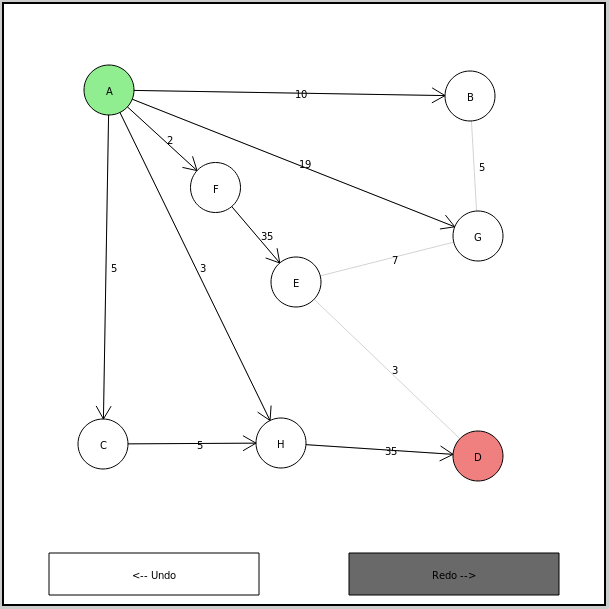
\includegraphics[width=0.7\linewidth]{/graphdrawer/dijkstraui}
    \caption{Dijkstra - user interface}
    \label{fig:graphdrawerDijkstraUserInterface}
\end{figure}
If the Dijkstra controller is not given a configuration object, then it will only display a white screen without allowing any user interaction. This happens becuase this controller is made for finding the shortest path, or for showing how the algorithm finds the shortest path. It can not be used to create a graph. The following properties can be determined by the configuration object:
\begin{enumerate}
    \item \code{steps}, should be an array of the steps the algorithm uses to find the shortest path. This can be undefined, if the intention is for the student to use the algorithm to find the path. If \code{steps} is defined, then the \code{graph} configuration is not needed.
    \item \code{startColor}, the fill color used for the start node.
    \item \code{endColor}, the fill color used for the end node.
    \item \code{edgeColor}, is the color used for lines which show the path between nodes.
    \item \code{graph}, contains information about the graph which the student should use the algorithm on. The following list is all of the possible properties on the \code{graph} object.
    \begin{itemize}
        \item \code{graph}, contains the graph.
        \item \code{from}, should be the starting node.
        \item \code{to}, should be the end node.
        \item \code{nodes}, should be an array of node objects which the graph consists of.
    \end{itemize}
\end{enumerate}
The Dijkstra controller uses the steps array to store operations. There are three step types:
\begin{enumerate}
    \item \code{"Initial"}, is used to store information about the graph. It has the same properties as the \code{graph} configuration object.
    \item \code{"Distance"}, is used to show that the algorithm is checking the cost between to nodes. 
\end{enumerate}
